\documentclass{article}
\usepackage{graphicx}
\begin{document}
\section{Figures}
\begin{figure}[h]
\centering
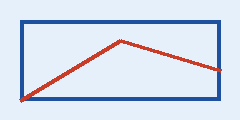
\includegraphics[width=0.5\textwidth]{figs/wide.png}
\caption{A wide image}\label{fig:wide}
\end{figure}

\begin{figure}[h]
\centering

\includegraphics[width=3cm]{figs/photo}
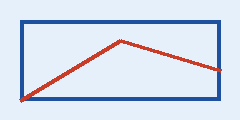
\includegraphics[height=1in]{figs/wide.png}
\caption{Two images, one reused}\label{fig:two}
\end{figure}

Inline 
\includegraphics[width=\linewidth]{figs/photo.jpg} and natural size 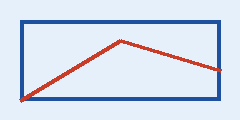
\includegraphics{figs/wide.png}.

\begin{figure}[h]
\centering

\includegraphics{figs/vector.pdf}
\caption{Vector figure}
\end{figure}

\includegraphics{figs/missing.png}

\begin{tabular}{ll}
Image & 
\includegraphics[width=1cm]{figs/photo.jpg} \\
\end{tabular}

See Figures \ref{fig:wide} and \ref{fig:two}.
\end{document}
